%!TEX root = ../thesis.tex
\section{Posters}\label{app_sec:posters}

%%%%%%%%%%%%%%%%%%%%%%%%%%%%%%%%%%%%%%%%%%%%%%%%%%%%%%%%%%%%%%%%%%%%%%%%%%%%%%%%%%%%%%%%%%%%%%
\Communication{Poster} {Towards Exoplanet Atmospheres: new data reduction for the \nir{}}% Title
% Type: Seminar/Talk/Poster
{2014, July 17--27}% Date
{\textit{IVth Azores International Advanced School in Space Sciences}, Horta, Faial, Azores Islands, Portugal}% Location
{http://www.iastro.pt/research/conferences/faial2016/}% Website
{}% Points
{In this poster I outline the goal of the direct subtraction technique, detailing the data preparation and correct steps needed. It shows the first results of applying the direct subtraction on our observations. The poster is provided on the next page.}% Description


%%%%%%%%%%%%%%%%%%%%%%%%%%%%%%%%%%%%%%%%%%%%%%%%%%%%%%%%%%%%%%%%%%%%%%%%%%%%%%%%%%%%%%%%%%%%%%
\Communication{Poster} {Towards Exoplanet Atmospheres: new data reduction for the \nir{}}% Title
% Type: Seminar/Talk/Poster
{2016, Sept. 09}% Date
{\textit{XXVI Encontro Nacional de Astronomia e Astrofísica (ENAA)}, Aveiro, Portugal}% Location
{ http://gravitation.web.ua.pt/enaa2016/index2a62.html?q=node/3}% Website
{20}% Points
{I presented the same poster at ENAA as I did at the IVth Azores International Advanced School in Space Sciences.}


%{\centering 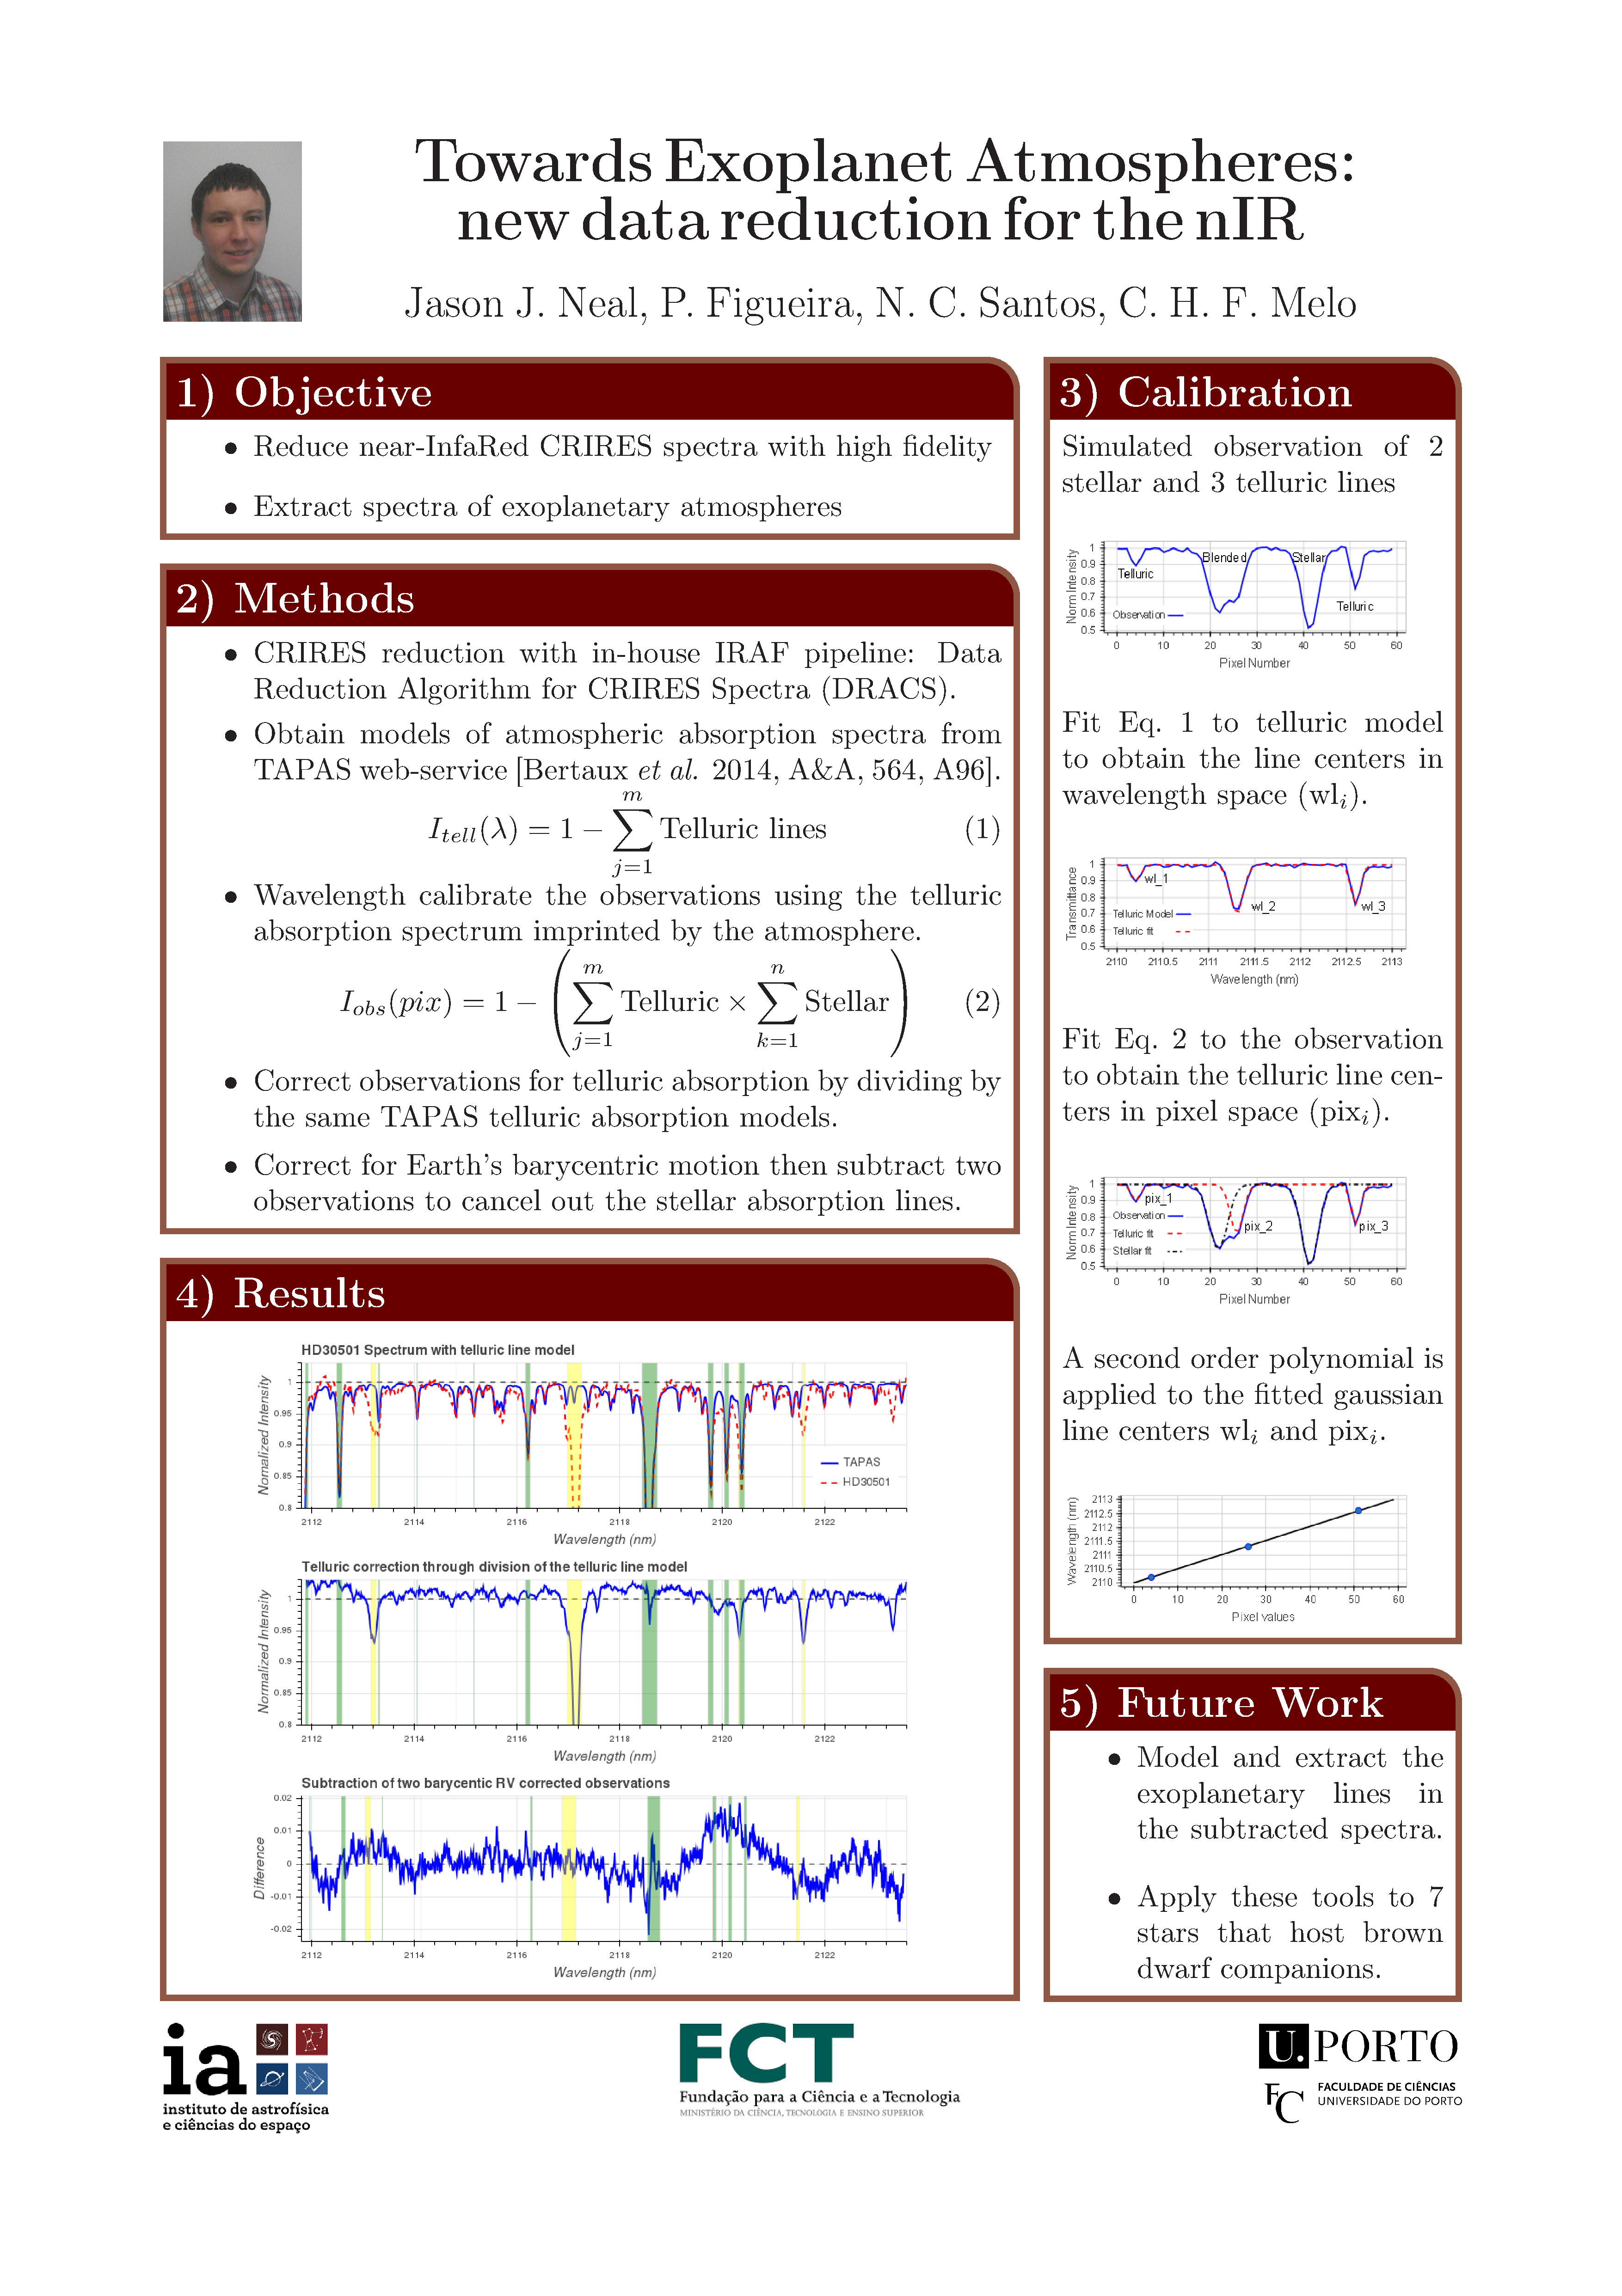
\includegraphics[width=0.97\textwidth, keepaspectratio=true, page = 1, trim = 1.5cm 1cm 1.5cm 1cm, clip = true]{appendices/papers/Azores2016_Final}}
{\centering 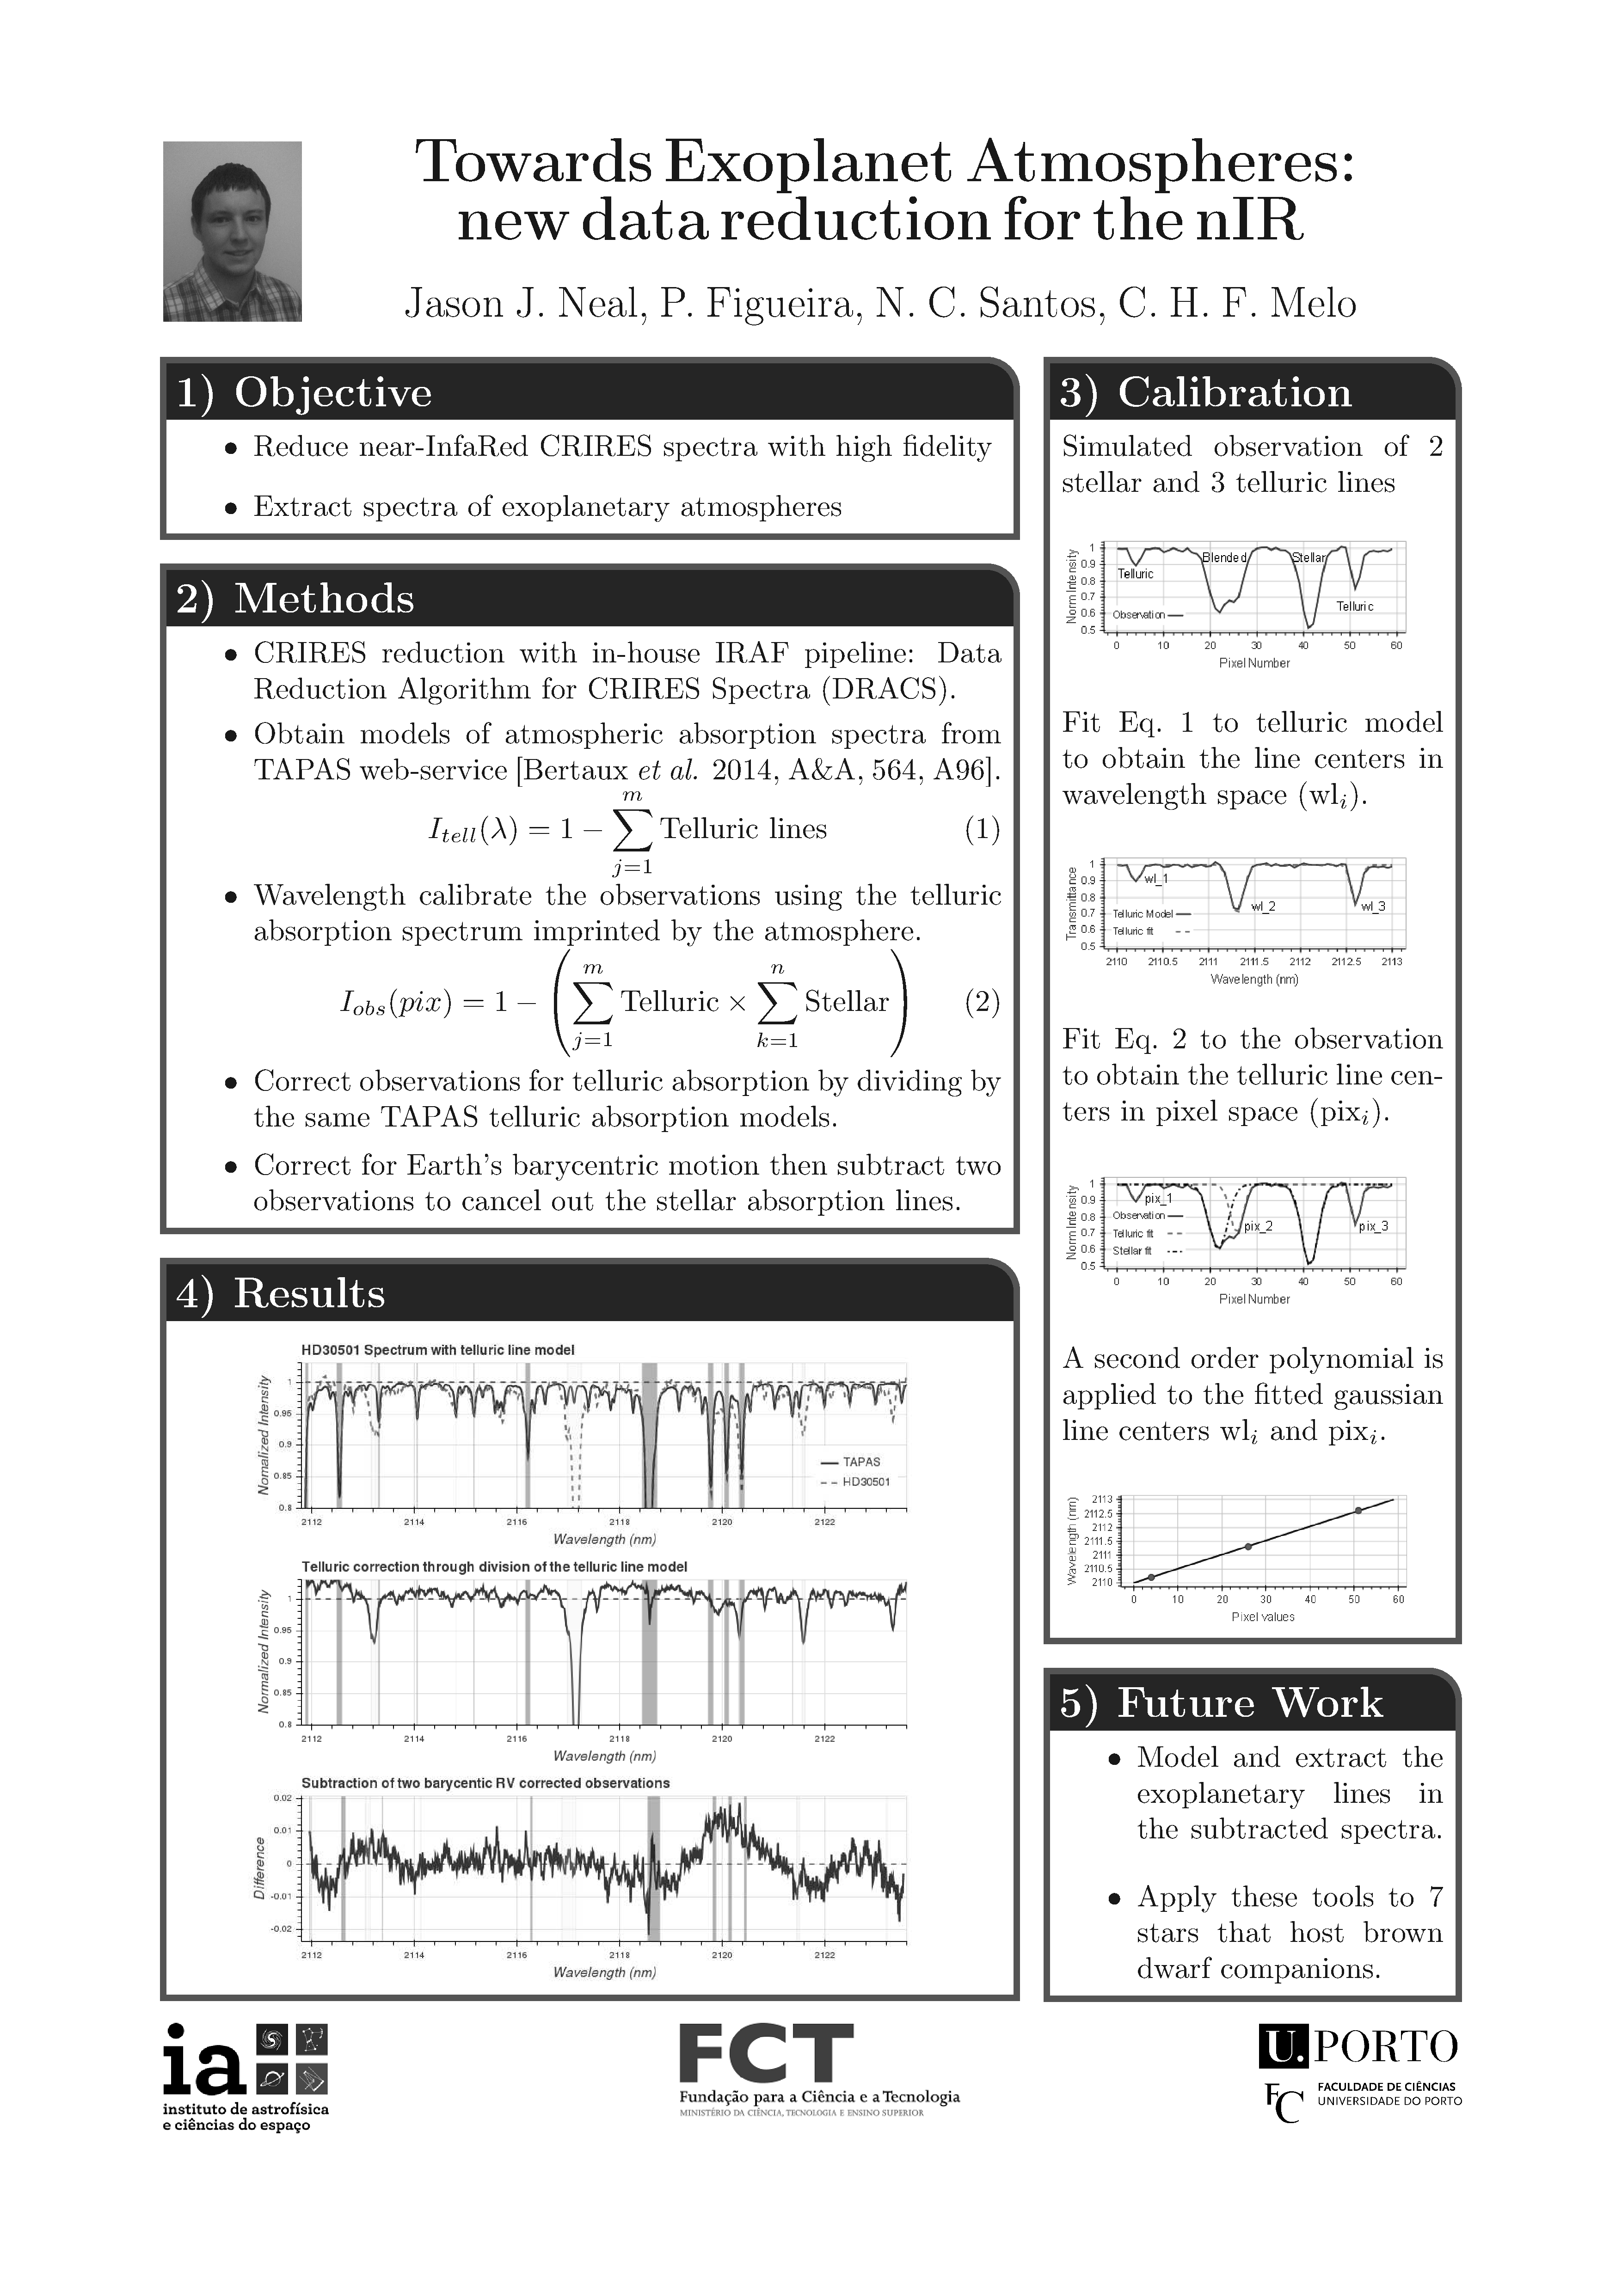
\includegraphics[width=1\textwidth, keepaspectratio=true, page = 1, trim = 1.5cm 1cm 1.5cm 1cm, clip = true]{appendices/papers/Azores2016_grey}}